%****************************************************************
% Chapter X
%****************************************************************
\label{chapter-technology}
\chapter{Technology}

This chapter expose how I am going to discover geographic data visualization in a 3D virtual reality world by presenting some of the main technologies used in this project, along with the reason why they are suited to my aims.

%****************************************************************
\section{Android Phone}

There are reasons we implemented this project on the Android device. We intent to build the virtual reality on a common and familar device in the world. Smartphone is fully deserve the title that not only it has a incredible fast growth trend in the last decade and a good promising prospect, but also they have built-in sensors that measure motion, orientation, and various environmental conditions. These sensors are capable of providing raw data with high precision and accuracy, and are useful to monitor three-dimensional device movement or positioning.

\begin{figure}[H]
\caption[smartphone-shipments-forecast]{Global Smartphone Shipments Forecase \parencite{td.global-smartphone-market.2015}}
\label{fig:smartphone-shipments-forecast}
\centering
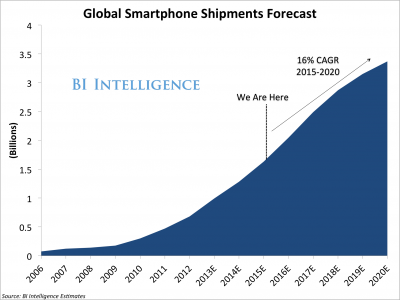
\includegraphics[width=\linewidth]{Figures/smartphone-shipments-forecast.png}
\decoRule
\end{figure}

According to data from the International Data Corporation (IDC), Android dominated the smartphone market with a share of 87.6\% in the worldwide.

\begin{figure}[H]
\caption[smartphone-os-market-share]{Smartphone OS Market Share \parencite{idc.smartphone-os-market-share.2016}}
\label{fig:smartphone-os-market-share}
\centering
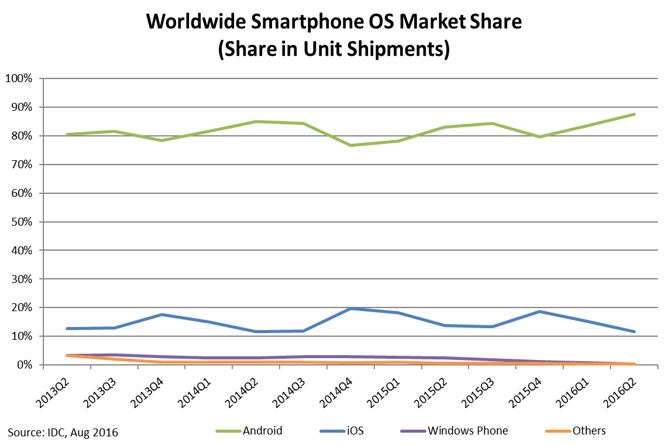
\includegraphics[width=\linewidth]{Figures/smartphone-os-market-share.png}
\decoRule
\end{figure}

Moreover, the perfect part is the Google VR SDK \parencite{google.vr-sdk.2016} for Android supports and the affordable Cardboard product \parencite{google.cardboard.2016} designed for different kind of mobile devices.

%****************************************************************
\section{OpenGL ES}

Android includes support for high performance 2D and 3D graphics with the Open Graphics Library, specifically, the OpenGL ES API \parencite{google.opengles.2016}. OpenGL ES is a flavor of the OpenGL specification intended for embedded devices. Android supports several versions of the OpenGL ES API:

\begin{table}[H]
\caption{OpenGL ES API specification supported by Android}
\label{tab:opengles-spec-android}
\centering
\begin{tabular}{l l l}
\toprule
\tabhead{OpenGL ES Version} & \tabhead{Android Version}\\
\midrule
OpenGL ES 1.0 & Android 1.0 and higher\\
OpenGL ES 1.1 & Android 1.0 and higher\\
OpenGL ES 2.0 & Android 2.2 (API level 8) and higher\\
OpenGL ES 3.0 & Android 4.3 (API level 18) and higher\\
OpenGL ES 3.1 & Android 5.0 (API level 21) and higher\\
\bottomrule
\end{tabular}
\end{table}

%****************************************************************
\section{Keyhole Markup Language}

We were looking for a simple markup languages that we can publish and consume data  in interoperable formats without the need for technical assistance.

In this section, we present Keyhole Markup Language (KML) \parencite{Google.kml.2016}, a file format to display geographic data ( (Note that KML files can be combined with other supporting files such as imagery in a zip archive, producing a KMZ file). It is an international standard maintained by the Open Geospatial Consortium, Inc. (OGC), and also it is supported by many Virtual Globes (VG) applications and other GIS systems and is therefore already becoming a de facto standard. Such as the most wellknown VG application Google Earth that has the largest community, NASA World Wind has more focus toward scientific users, and ArcGIS Explorer that is a lightweight client to the ArcGIS Server \parencite{blower.sharing-visualizing.2007}.

From an environmental science point of view, KML is a somewhat limited language. It describes only simple geometric shapes on the globe (points, lines and polygons) and is not extensible. It is, in many respects, analogous to Geography Markup Language (GML) 3.0+ is much more sophisticated and allows the rich description of geospatial features such as weather fronts and radiosonde profiles. So, KML is currently not suitable as a fully-featured, general-purpose environmental data exchange format.

Figure \ref{fig:kml-schema} shows the KML schema. From the point of view of usability, KML spans a gap between very simple (e.g. GeoRSS) and more complex (GML) formats, that makes it easy for non-technical scientists to share and visualize simple geospatial information which can then be manipulated in other applications if required. Also it makes it easier for user to visualize their data quickly using a single, simple data file. Moreover, its rapidly-growing adoption by scientists, and it is important to be aware of that virtual geographic data visualization (and KML) do not attempt to replace more sophisticated systems. 

\begin{figure}[H]
\caption[kml-schema]{KML schema \parencite{Google.kml.2016}}
\label{fig:kml-schema}
\centering
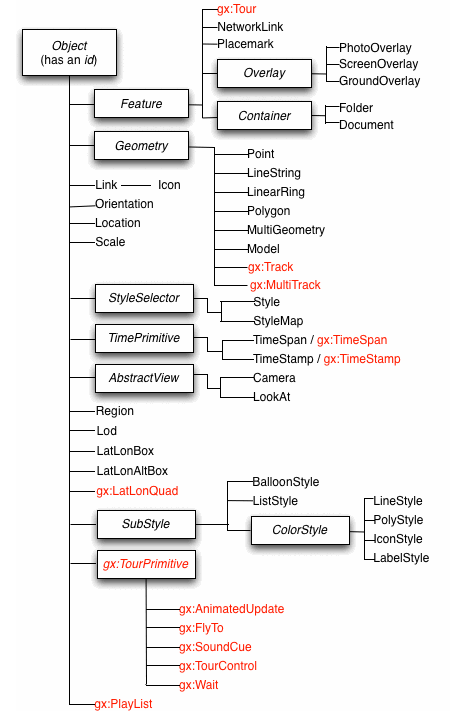
\includegraphics[height=0.5\textheight]{Figures/kml-schema.png}
\decoRule
\end{figure}

%****************************************************************
\section{Network}
\label{section:network}

The key strengths of virtual reality applications is not only easy-to-use, and intuitive nature, but also the ability to incorporate new data very easily. Therefore, real-time data are very important in the environmental sciences \parencite{blower.sharing-visualizing.2007}. To do that, a web server is needed. In this project, we implemented a RESTful web server to support communication with client, along with a  file server to synchronize data. In the client side.

Go (often referred to as golang \parencite{google.golang.2016}) is an open source programming language, and it is compiled, concurrent, garbage-collected, statically typed language developed at Google in late 2007. It was conceived as an answer to some of the problems we were seeing developing software infrastructure \parencite{google.talk-golang.2012}. Also, it growing fast that each month the contributors outside Google is already more then contributors inside the Go team. 

We are using Go to build the server, it is well suited for developing RESTful API’s. The net/http standard library provides key methods for interacting via the http protocol. On the other hand, since our client is Android phone, we introduced Volley for transmitting network data (Volley is an open sourced HTTP library that makes networking for Android apps easier and most importantly, faster \parencite{google.volley.2016}), and jsoup (Java HTML Parser \parencite{joup.2016}) for analysing HTML format response.

%****************************************************************
